\documentclass[crop,tikz]{standalone}% 'crop' is the default for v1.0, before it was 'preview'

\usepackage{pgfplots}
\usepackage{pgfplotstable}
\pgfplotsset{compat=newest}

\usetikzlibrary{patterns}
\usetikzlibrary{matrix}
\usetikzlibrary{positioning}
\usetikzlibrary{arrows.meta}
\usetikzlibrary{fit}
\usetikzlibrary{math}
\usetikzlibrary{calc}
\usetikzlibrary{backgrounds}
\usetikzlibrary{decorations.pathmorphing}
\usetikzlibrary{decorations.markings}
\usetikzlibrary{pgfplots.groupplots}

\tikzset{
  midarrow/.style={draw, postaction={decorate},
  decoration={markings,mark=at position .55 with {\arrow[draw]{>}}}},
  midarrow-rev/.style={draw, postaction={decorate},
  decoration={markings,mark=at position .55 with {\arrow[draw]{<}}}},
  midarrow-dashed/.style={draw, dashed, postaction={decorate},
  decoration={markings,mark=at position .55 with {\arrow[draw]{>}}}},
  midarrow-dashed-thick/.style={
    draw, thick, dashed, postaction={decorate},
  decoration={markings,mark=at position .50 with {\arrow[draw]{>}}}},
}
\tikzset{
  TT/.style={decorate, draw=black,
  decoration={coil,aspect=0.7,segment length=3.2pt,amplitude=2pt}}
}
\tikzset{
  sigma/.style={dashed}
}

\usepgfplotslibrary{groupplots} % Libraries to generate group plots



\begin{document}
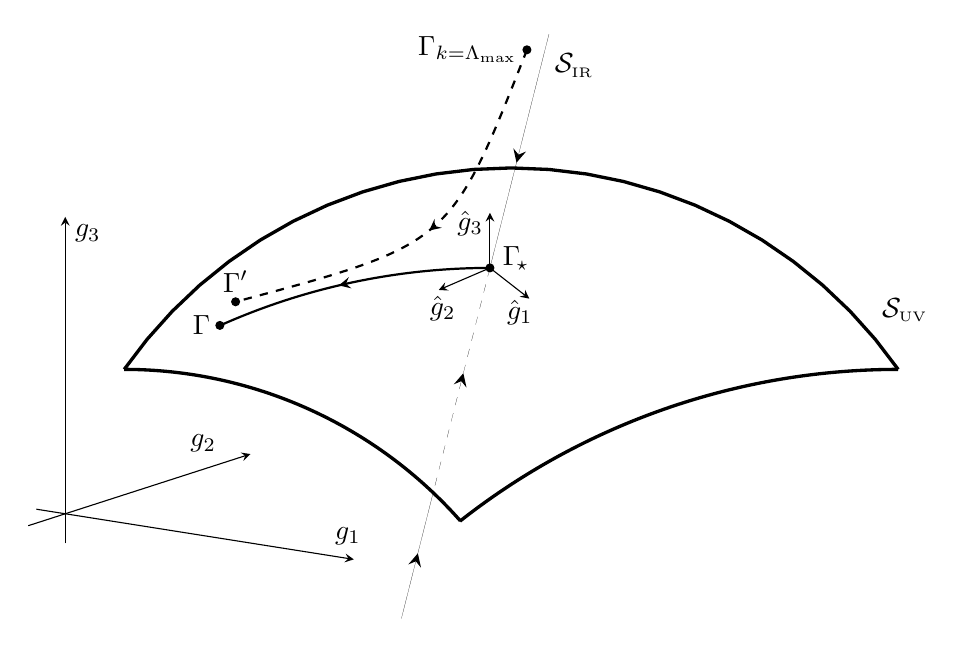
\begin{tikzpicture}[
  >=stealth,
  scale=1.00,
  ]

  \tikzmath{
    \radius    = 6.00; % radius of the circle for UV critical surface
    \radiusa   = 1.5*\radius; % radius of the circle for UV critical surface
    \radiusb   = 0.95*\radius; % radius of the circle for UV critical surface
    \degs      = 35;
    \degsinv   = 180-\degs;
    \dotradius = 0.05; % radius of the circles that make the dots
    \basex     = 6.5;
    \basey     =-0.5;
  }

  \coordinate (base)          at ( \basex, \basey );
  \coordinate (insetPosition) at ( 4.60, 3.80 );
  \coordinate (lower)         at (-0.43, 1.02 );
  \coordinate (FP)            at ( 6.23, 4.23 );
  \coordinate (Gamma)         at ( 2.80, 3.50 );
  \coordinate (dirx)          at ( 0.50,-0.39 );
  \coordinate (diry)          at (-0.65,-0.28 );
  \coordinate (dirz)          at ( 0.00, 0.70 );
  \coordinate (SUV)           at (11.50, 3.70 );
  \coordinate (SIR)           at ( 7.30, 6.80 );
  \coordinate (IR)            at ( 0.75, 2.97 );
  \coordinate (A)             at ( 6.70, 7.00 );
  \coordinate (B)             at ( 3.00, 3.80 );
  \coordinate (controlAB)     at ( 5.73, 4.53 );

  % The main coordinate system
  \begin{axis}[
    view={35}{15},
    axis lines=center,
    ticks=none,
    xmin=-.5,
    xmax=5,
    ymin=-1,
    ymax=5,
    zmin=-.5,
    zmax=5,
    xlabel={$g_1$},
    ylabel={$g_2$},
    zlabel={$g_3$},
    ]
  \end{axis}

  % The UV critical surface itself
  \draw[very thick,domain=\degs:\degsinv] plot ({\radius*cos(\x)+\basex}, {\radius*sin(\x)+\basey});
  \draw[very thick,] ($ (base) + ({ cos(\degs)*\radius}, {sin(\degs)*\radius}) $) arc (90:128.2:\radiusa);
  \draw[very thick,] ($ (base) + ({-cos(\degs)*\radius}, {sin(\degs)*\radius}) $) arc (90: 41.5:\radiusb);

  % The FP with annotation
  \draw[fill] (FP) circle [radius=\dotradius];
  \node at ($ (FP) + (0.33, 0.12) $) {$\Gamma_{\!\star}$};

  % The small (diagonalised) coordinate system
  \draw[->] (FP) -- ($ (FP) + (dirx) $);
  \node at ($ (FP) + ( 0.38,-0.57) $) {$\hat g_1$};
  \draw[->] (FP) -- ($ (FP) + (diry) $);
  \node at ($ (FP) + (-0.60,-0.52) $) {$\hat g_2$};
  \draw[->] (FP) -- ($ (FP) + (dirz) $);
  \node at ($ (FP) + (-0.25, 0.56) $) {$\hat g_3$};

  % Annotation UV and IR critical surface
  \node at (SUV) {$\mathcal S_{\scriptscriptstyle{\mathrm{UV}}}$};
  \node at (SIR) {$\mathcal S_{\scriptscriptstyle{\mathrm{IR}}}$};

  % IR critical surface
  \draw[
  postaction={decorate},
  decoration={markings, mark=at position .55 with {\arrow[scale=2]{>}}},
  line width=0.02mm,
  ] ($ (FP) + (IR) $) -- (FP);
  \draw[
  dashed,
  postaction={decorate},
  decoration={markings, mark=at position .55 with {\arrow[scale=2]{>}}},
  line width=0.02mm,
  ] ($ (FP) - (IR) $) -- (FP);
  \draw[
  postaction={decorate},
  decoration={markings, mark=at position .55 with {\arrow[scale=2]{<}}},
  line width=0.02mm,
  ] ($ (FP) - (IR) $) -- ($ (FP) - 1.5*(IR)$);

  % fundamental theory, with trajectory and dot
  \draw[fill] (Gamma) circle [radius=\dotradius] node[left] {$\Gamma$};
  \draw[midarrow, thick] (FP) arc (90:114:1.4*\radius);

  % Effective trajectory
  \draw[fill] (A) circle [radius=\dotradius]
  node[left] {$\Gamma_{k=\Lambda_{\mathrm{\scriptscriptstyle{max}}}}$};
  \draw[fill] (B) circle [radius=\dotradius]
  node[above] {$\Gamma'$};
  \draw[midarrow-dashed-thick] (A)  .. controls (controlAB) .. (B);

\end{tikzpicture}
\end{document}
